\documentclass{cshonours}

\usepackage{graphics}  % For figures
\usepackage{amsmath}   % For mathematical expressions
\usepackage{amssymb}   % For mathematical symbols
\usepackage{booktabs}  % For professional tables
\usepackage{array}     % For advanced column formatting
\usepackage{tabularx}  % For tables of a specific width
\usepackage{threeparttable} % For tables with notes
\usepackage{adjustbox} % To adjust box content (e.g., scale table)
\usepackage{makecell}  % For multi-line cells
\usepackage{subcaption}


\newcolumntype{L}{>{\raggedright\arraybackslash}X}
\newcolumntype{C}[1]{>{\centering\arraybackslash}p{#1}}

\title{Temporal Geometric Neural Networks for Rumour Detection: Architectures, Applications, and Temporal Nuance}
\author{[Matthew Haskins]}

\keywords{Graph Neural Networks, Temporal Graph Neural Networks, Graph Attention Network, Dynamic Graphs, Rumour Detection, Social Network Analysis, Misinformation, Temporal Attention, PHEME Dataset}
\categories{I.2.6, H.2.8} % Computing methodologies - AI and Database applications - Data mining

\begin{document}
\maketitle

\begin{abstract}

\emph{Rumour detection} on social media hinges on recognising \emph{how} information propagates, not merely \emph{what} is said. To probe the role of temporal dynamics, we benchmark six graph-based neural models on the \emph{PHEME} Twitter corpus: static \emph{GCN}, \emph{GAT}, \emph{GATv2}, and three dynamic variants-\emph{DySAT}, a \emph{simplified DySAT} without temporal self-attention, and the continuous-time \emph{Temporal Graph Network} (TGN). Results show that temporal self-attention is valuable but not transformative: full DySAT edges out its aggregation-only ablation by roughly 3 percentage points in macro-F1, confirming that fine-grained time weighting helps but that much of the signal is already captured by simpler temporal aggregation. By contrast, TGN fails to surpass even our static graph baseline, suggesting that its memory-update mechanism is ill-suited to PHEME's sparse, subtle temporal cues. Among static methods, \emph{GATv2} delivers a consistent yet modest improvement over GAT, illustrating the benefit of more expressive attention even without explicit temporal modelling. Qualitative assessments of t-SNE projections further reveal that temporal models carve cleaner rumour/non-rumour clusters than static ones, underscoring a geometric advantage. Collectively, these findings indicate that effective rumour detection benefits from architectures that embed temporal reasoning directly, while also cautioning that not all continuous-time designs transfer cleanly to real-world social datasets. 

\end{abstract}


\tableofcontents
\listoffigures

\chapter{Introduction}

False or unverified claims now surge through social media with unprecedented speed and reach, shaping public opinion and even real-world behaviour~\cite{vosoughi2018spread}.  Twitter conversation threads, in particular, unfold as intricate cascades of replies and retweets whose topology and timing encode valuable clues about credibility.  The \emph{PHEME} corpus captures this phenomenon across major breaking-news events, providing thread-level labels that distinguish rumours from non-rumours~\cite{zubiaga2016pheme}.  Yet despite a decade of progress, automatic rumour detection remains challenging because it must parse both the \emph{content} of posts and the \emph{dynamics} of their propagation.


Graph Neural Networks (GNNs) offer a principled way to exploit the relational context of social conversations, propagating information along reply or retweet links so that each node embedding reflects its neighbourhood \cite{kipf2017semi}.  Early static models such as GCN and Bi-GCN already outperform text-only baselines on PHEME by modelling conversation structure \cite{bian2020rumor}, while attention-based variants (GAT) capture heterogeneous neighbour importance \cite{lv2022rumor}.  However, these approaches compress a dynamic process into a single snapshot, discarding temporal patterns that differentiate false from factual narratives-patterns documented at scale by Vosoughi and colleagues \cite{vosoughi2018spread} and echoed across subsequent misinformation studies \cite{survey2024disinfo}.


To reincorporate time, researchers have proposed two main paradigms.  \emph{Snapshot-based self-attention}, exemplified by \emph{DySAT}, learns joint structural-temporal attention over a sequence of graph slices, enabling nodes to weigh past states adaptively \cite{sankar2020dysat}.  At the other extreme, \emph{continuous-time memory} models such as the \emph{Temporal Graph Network} (TGN) update per-node memories at every interaction event, supporting fine-grained streaming inference \cite{rossi2020tgn}.  More recently, \emph{GATv2} extends static attention with query-dependent weights, narrowing the expressiveness gap between time-agnostic and time-aware designs \cite{brody2022gatv2}.


Although temporal mechanisms are intuitively appealing, their real-world benefit is still an open question.  The literature reports substantial gains for DySAT on link-prediction benchmarks \cite{sankar2020dysat} and for TGN on interaction forecasting \cite{rossi2020tgn}, yet evidence from rumour detection is limited and sometimes contradictory \cite{liu2024rumor}.  Moreover, the additional complexity-larger hyper-parameter spaces, heavier computation, and harder interpretability-may not justify modest accuracy improvements \cite{survey2024disinfo}.  A systematic comparison on a common benchmark is therefore needed.


Leveraging the modular \emph{Araneos} platform, developed during the course of this research, we perform the first head-to-head evaluation of six representative architectures-GCN, GAT, GATv2, DySAT, a simplified DySAT without temporal attention, and TGN-on identical PHEME conversation graphs.  This design isolates the impact of temporal mechanisms embedded in model structure rather than in handcrafted features or data splits.  The investigation is guided by three questions:

\begin{enumerate}
    \item \emph{RQ1:} Do temporal GNNs achieve materially better rumour-detection performance than strong static counterparts on PHEME?  
    \item \emph{RQ2:} How much improvement, if any, does DySAT's temporal self-attention deliver relative to simple temporal aggregation?  
    \item \emph{RQ3:} Why might a continuous-time memory model like TGN fail to outperform static baselines despite its success on other dynamic-graph tasks?  
\end{enumerate}


Addressing these questions advances both theory and practice.  Theoretically, it clarifies whether temporal reasoning should be baked into the \emph{architecture} of rumour-detection systems or can be emulated with richer static features and expressive attention \cite{choi2021dynGCN}.  Practically, it informs platform engineers who must balance detection accuracy against computational cost and interpretability-critical factors for real-time moderation pipelines \cite{survey2024disinfo}.  By exposing the conditions under which temporal dynamics help or hinder, this work charts a more evidence-based path toward trustworthy, scalable misinformation defences.


\chapter{Background}\label{chap:background}

Rumour detection occupies a nexus of natural-language understanding, network science, and temporal data analysis.  A single Twitter thread weaves together user roles, linguistic stance, and the high-velocity cascade by which information fans out across the platform.  Over roughly ten years, the research community has pursued this multilayered signal through five overlapping neural ``eras.''  Each era offered a sharper lens but also revealed fresh blind spots, ultimately pointing toward Temporal Graph Neural Networks (TGNNs)-the architectural family whose strengths and open questions motivate the experiments in this thesis.  This chapter retraces that trajectory, formalises core graph-learning concepts for readers versed in mainstream deep learning, and establishes the conceptual bridge to the dedicated literature review that follows.  

Figure \ref{fig:timeline} summarises the milestones, while Figure \ref{fig:temporal_overview} previews how temporal GNNs extend static message passing.

%%%%%%%%%%%%%%%%%%%%%%%%%%%%%%%%%%%%%%%%%%%%%%%%%%%%%%%%%%%%%%%%
\begin{figure}[htbp]
  \centering
  \includegraphics[width=\textwidth]{../figures/rumour_timeline.pdf}
  \caption[Evolution of neural approaches to rumour detection]{\textit{Evolution of neural approaches to rumour detection.  Text-sequence models led to contextual language models; propagation-aware hybrids introduced handcrafted graph cues; static Graph Neural Networks (GNNs) unified content and structure; Temporal GNNs embed timing directly in the learning process.}}
  \label{fig:timeline}
\end{figure}
%%%%%%%%%%%%%%%%%%%%%%%%%%%%%%%%%%%%%%%%%%%%%%%%%%%%%%%%%%%%%%%%

\section{From Sequential to Structural Thinking}

Early neural systems framed rumour detection as a purely \emph{sequential} problem: RNNs and CNNs scanned token streams \cite{yu2017cnn}, and later Transformers further enlarged the lexical receptive-field \cite{rahman2024primer}. Yet these models implicitly flattened the social conversation-reply trees, user interactions, temporal retweets-into a one-dimensional string, forcing researchers to bolt on handcrafted graph features that only partially captured how misinformation diffuses. Because a rumour's credibility often hinges on \emph{who} shares it, \emph{when}, and along \emph{which} relational paths, the research community pivoted toward a \emph{structural} view: Graph Neural Networks (GNNs) treat users as nodes, interactions as edges, and learn to pass messages along the very propagation channels that make rumours viral \cite{bian2020rumor}. This shift unifies textual semantics with network topology in a single differentiable framework, delivering better generalisation across events and platforms while eliminating brittle feature engineering. 
\section{Graph Neural Networks: A Unified Structural Lens}


Let a directed graph be \(G=(V,E)\) with \(|V|=N\) nodes and \(|E|\) edges.  Each node \(v\in V\) carries an initial feature vector \(\mathbf{x}_v\in\mathbb{R}^{d_0}\); edges may hold attributes \(\mathbf{e}_{uv}\).  In a social-media conversation, nodes can represent tweets, users, or both; edges encode reply, retweet, or mention relationships.  The adjacency matrix \(A\) (or sparse edge list) captures topology, while a timestamp \(t_{uv}\) records when edge \((u,v)\) occurred.


Most contemporary GNNs follow the Message-Passing Neural Network (MPNN) template.  For layer \(l\) and node \(i\),
\begin{equation}
\mathbf{h}_i^{(l+1)}
=\sigma\!\Bigl(
f_{\text{comb}}\!\bigl(
\mathbf{h}_i^{(l)},\;
f_{\text{agg}}\bigl\{
g_{\text{msg}}\!\bigl(
\mathbf{h}_i^{(l)},\mathbf{h}_j^{(l)},\mathbf{e}_{ij}\bigr)
\; : j\!\in\!\mathcal{N}(i)\bigr\}\bigr)
\Bigr),
\label{eq:mpnn}
\end{equation}
where  
\(g_{\text{msg}}\) maps an edge to a message,  
\(f_{\text{agg}}\) is permutation invariant (sum, mean, max, attention),  
\(f_{\text{comb}}\) fuses aggregated evidence with the node state,  
and \(\sigma\) is an activation \cite{gnn_applications_2024}.  
Stacking \(L\) layers yields embeddings that capture up-to-\(L\)-hop structural context.


The Graph Convolutional Network (GCN) instantiates Eq.~\eqref{eq:mpnn} by using  
\(g_{\text{msg}}(\mathbf{h}_j)=\mathbf{h}_j\),  
\(f_{\text{agg}}=\textstyle\sum\nolimits_{j}\tilde{D}^{-1/2}\tilde{A}_{ij}\tilde{D}^{-1/2}\mathbf{h}_j\),  
and \(f_{\text{comb}}(\cdot)=W^{(l)}(\cdot)\) \cite{kipf2017semi}.  
The symmetric normalisation \(\tilde{D}^{-1/2}\tilde{A}\tilde{D}^{-1/2}\) ensures each message is weighted by node degree, providing a spectral approximation of Laplacian smoothing.  In rumour detection, Bi-GCN extended this principle by separating top-down from bottom-up propagation along conversation trees, yielding state-of-the-art F\(_1\) above 0.89 on Twitter15/16 datasets and 0.802 on PHEME \cite{bian2020rumor}.


Graph Attention Networks (GAT) replace fixed degree weights with learned coefficients  
\(\alpha_{ij}=\text{softmax}_j\bigl(\text{LeakyReLU}(\mathbf{a}^\top[W\mathbf{h}_i\|\;W\mathbf{h}_j])\bigr)\),  
allowing each node to emphasise informative neighbours and dampen noise \cite{velickovic2018gat}.  GATv2 removes the static key-query ordering, granting full query-adaptive weights and provably higher expressiveness \cite{brody2022gatv2}.  In practice, attention heat-maps often highlight authoritative denials or sceptical users, offering interpretability absent from sequence models.


Despite unifying content and structure, static GNNs freeze time.  They cannot differentiate a rumour that explodes and dies within an hour from one diffusing slowly but reaching comparable breadth.  Empirically, spread velocity, burstiness, and correction latency strongly distinguish misinformation from factual news \cite{vosoughi2018spread}.  Further, deep message passing can \emph{over-squash} long-range signals into fixed-width embeddings, hampering reasoning across many hops \cite{oversquashing_gnn_2023}.  Finally, the representational power of standard MPNNs is bounded by the first-order Weisfeiler-Lehman test \cite{xu2019gin}, restricting discrimination of topologically similar yet temporally divergent cascades.


\section{Temporal Graph Neural Networks}


A \emph{temporal} or \emph{dynamic} graph augments \(E\) with a timestamp map  
\(\tau:E\!\to\!\mathbb{R}_{\ge0}\).  
Learning tasks can model discrete ``snapshots'' \(G_1,\dots,G_S\) sampled at interval \(\Delta t\) or continuous-time event streams where each edge arrives asynchronously.  Rumour cascades exhibit both coarse timeline stages (breaking, correction, decay) and fine-grained micro-interactions (reply chains firing within seconds), making temporal modelling attractive.


Recent surveys categorise TGNNs along two axes \cite{dynamic_gnn_survey_2024}:  

\begin{enumerate}
\item \emph{Snapshot-based} methods process an ordered sequence of graphs and often apply attention to weigh historical snapshots.  
\item \emph{Continuous-time} methods update node states upon each event via time-aware memories or point-process kernels.
\end{enumerate}

The remainder of this thesis evaluates representative architectures from both families-DySAT (snapshot self-attention) and TGN (continuous-time memory)-because they capture complementary inductive biases that may benefit rumour detection.

\paragraph{DySAT (snapshot self-attention).}
DySAT introduces dual self-attention:  
structural attention learns intra-snapshot importance, while temporal attention learns which historical snapshots matter when predicting node states \cite{sankar2020dysat}.  
This design captures both local neighbourhood influence and overarching temporal evolution.

\paragraph{TGN (continuous-time memory).}
Temporal Graph Networks associate each node with a recurrent memory.  
Upon receiving an event \((u,v,t)\), time-encoded messages update memories \(\mathbf{m}_u,\mathbf{m}_v\); a readout module then combines memory and static features to produce on-the-fly embeddings \cite{rossi2020tgn}.  
Such memory systems support millisecond-level resolution and naturally model irregular interaction gaps.


Rumour cascades exhibit temporal signatures such as rapid early diffusion, late mass corrections, or user-credibility shifts over time.  Snapshot attention can weigh such phases differently, while continuous-time memories can reflect recency effects (e.g.\ ``fresh'' corrections damp rumour credibility more than stale ones).  Evaluating both paradigms therefore illuminates whether temporal granularity or modelling mechanism drives performance on PHEME.

%%%%%%%%%%%%%%%%%%%%%%%%%%%%%%%%%%%%%%%%%%%%%%%%%%%%%%%%%%%%%%%%
\begin{figure}[htbp]
  \centering
  \includegraphics[width=.9\textwidth]{../figures/static_vs_temporal.pdf}
  \caption[Static vs.~temporal processing]{\textit{Static vs.~temporal processing.  (a) Static GNN views a single aggregated graph. (b) DySAT applies structural \emph{and} temporal self-attention across ordered snapshots. (c) TGN streams individual events and updates node memories in continuous time.  Both paradigms aim to preserve timing cues lost in static aggregation.}}
  \label{fig:temporal_overview}
\end{figure}
%%%%%%%%%%%%%%%%%%%%%%%%%%%%%%%%%%%%%%%%%%%%%%%%%%%%%%%%%%%%%%%%


The panorama above shows how each methodological generation sharpened the rumour-detection lens:  
text models decoded \emph{content}, hybrids injected handcrafted \emph{context}, static GNNs \emph{learned} context, and TGNNs finally weave \emph{time} into representation learning.  Yet questions remain: Which temporal paradigm works best for sparse, high-burst datasets such as PHEME?  Does temporal modelling truly outperform expressive static attention, or are gains confined to dense dynamic graphs?  The next chapter surveys specialised TGNN literature and positions those questions within current research frontiers.


\chapter{Literature Review}\label{chap:literature}

Building on the background trajectory, this chapter reviews prior approaches to rumour detection with a focus on how temporal dynamics have (or have not) been integrated. We synthesize related work in five thematic areas: early text-centric models, static graph-based models, emerging temporal GNN frameworks, prevailing evaluation practices, and considerations for interpretability and deployment. We conclude by identifying key gaps and tensions in the literature and linking them to our research questions.


\section{Text-Centric Origins of Rumour Detection}
Early efforts framed rumour detection strictly as a text-classification task.  Feature-engineered classifiers in the early 2010s (e.g.\ credibility cues, denial lexicons) struggled to generalise beyond their handcrafted rules \cite{castillo2011credibility}.  Around 2015 the field pivoted to neural sequence models that could learn representations directly from raw tweets.

\paragraph{Recurrent and convolutional baselines.}  
Ma \textit{et al.}~\cite{ma2016detecting} showed that an RNN over time-ordered tweets lifts PHEME accuracy by \(\sim\)10 pp versus a feature-based SVM; follow-ups added GAN-GRU training \cite{ma2021temporal} or CNN n-gram filters \cite{yu2017cnn}.  While these models exploit chronological context, they linearise the conversation: reply trees and retweet fan-outs-often crucial cues-remain invisible, leading to misclassifications when the text of a rumour resembles real news but its propagation pattern does not \cite{zubiaga2018survey}.

\paragraph{Contextual transformers and hybrid models.}  
Fine-tuned BERT classifiers push macro-F1 a further 3-5 pp on PHEME \cite{liu2025enhancing}, yet they, too, are sequence-bound and vulnerable to \emph{context mimicry} (malicious users imitating fact-check language) because they ignore network position \cite{rahman2024primer}.  To inject structural cues, researchers have bolted simple graph signals onto text encoders.  A hierarchical RNN with user/time features \cite{guo2018hierarchical} and a tree-recursive network that propagates hidden states up reply chains \cite{ma2018rvnn} each add roughly 2-5 pp F1, but rely on heuristics such as stance labels or user-reputation scores \cite{lukasik2019stance}.

These incremental gains make one conclusion clear: \emph{text alone is not sufficient}.  The relational dynamics of who replies or retweets whom carry decisive information-motivating the graph-based approaches discussed next.


\section{Static Structural Models: Graph-Based Rumour Classifiers}
A decisive shift occurred when researchers began modelling rumour cascades as \emph{graphs} of tweets and replies.  Propagating information along these edges lets a model exploit who-talks-to-whom, rather than treating posts as independent or merely sequential.

\paragraph{Graph convolutional networks (GCN).}
Adapting the Kipf \& Welling GCN \cite{kipf2017semi} to rumour trees, Bi-GCN \cite{bian2020rumor} aggregates messages both bottom-up and top-down.  On PHEME this raised macro-F1 from \(\sim\!0.26\) (sequential LSTM) to \(\sim\!0.47\) in leave-one-event-out tests-a 20 pp leap that highlights the value of structural cues such as wide, shallow sceptical branches versus deep chains of confirmations.  Later variants fused GCN with RNNs or user-post graphs \cite{wang2020satire}, but the central finding is consistent: adding the conversation graph yields large gains over text-only baselines.

\paragraph{Graph attention networks (GAT).}
GATs \cite{velickovic2018gat} weight neighbours unequally, letting the model focus on informative replies (e.g.\ eyewitnesses) and down-weight noisy retweets.  Rumour studies report modest bumps-typically 2-4 pp macro-F1 over vanilla GCN on Twitter$_{15/16}$ and PHEME \cite{lv2022rumor, patel2022rumour}.  Attention also aids interpretability, as salient edges align with human judgments of credible corrections.

\paragraph{GATv2 and recent refinements.}
GATv2 \cite{brody2022gatv2} replaces the fixed linear attention in GAT with a fully learnable function, increasing expressiveness without adding time awareness.  Although still little-tested for rumours, our Chapter 5 experiments show a small but consistent improvement over GAT on PHEME, suggesting richer intra-graph weighting helps close (but not erase) the gap to temporal models.

In sum, static GNNs-GCN, GAT, GATv2-demonstrate that structural context sharply boosts performance.  Yet by collapsing an unfolding cascade into a single snapshot they ignore \emph{when} interactions occur, motivating the temporal approaches surveyed next.


\section{Temporal GNN Families: Snapshot vs. Continuous-Time}
Motivated by the documented temporal patterns of misinformation spread (e.g., the speed and frequency differences observed by \cite{vosoughi2018spread}), recent work has explored graph neural networks that embed \emph{time dynamics} directly into their architecture. Broadly, two paradigms have emerged: (1) \emph{discrete-time models} that learn from a sequence of graph ``snapshots'' over time, and (2) \emph{continuous-time models} that process individual interaction events in temporal order. In this section, we focus on two representative frameworks from each family-\emph{DySAT} and \emph{TGN}-which are also the temporal GNNs evaluated in our experiments. We delve into how each encodes temporal information, their internal mechanisms (attention vs. memory), and what strengths or limitations have been noted, especially in the context of rumour data.

\section*{DySAT: Snapshot-based self-attention}

DySAT \cite{sankar2020dysat} learns node embeddings from a \emph{sequence} of graph snapshots, applying attention first within each snapshot (structural) and then across snapshots (temporal). Prior work shows that this dual attention lifts link-prediction AUC by roughly 3-5 pp over dynamic-RNN and static GCN baselines on generic benchmarks. In rumour detection, however, the gains are far more modest: studies that report DySAT on PHEME or Twitter$_{15/16}$ find only a 2-4 pp macro-F1 improvement over well-tuned static GCN/GAT variants, and sometimes none at all.  

The attraction of DySAT is its ability to weight past snapshots adaptively-capturing, for example, an early spike of engagement that signals a debunking burst-but it inherits classic snapshot pitfalls. Performance depends on the chosen interval (too coarse hides order, too fine amplifies noise), and self-attention across $K$ slices adds $O(K^2)$ cost. Because architectural details are covered in Chapter 4, we retain here only the empirical takeaway that \emph{temporal self-attention may help, but its effect size is contested}. To quantify this, our experiments in Chapter 5 compare full DySAT with a ``no-temporal-attention'' ablation, directly addressing \textbf{RQ2}.  

\section*{TGN: Continuous-time memory networks}

Temporal Graph Networks (TGN) \cite{rossi2020tgn} process each interaction in exact time order, updating a learnable memory for the nodes involved. This event-level design excels on dense interaction streams (e.g.\ Reddit or financial networks) where repeated edges let memory accumulate; on such data TGN often exceeds static GNNs by 5-10 pp in link prediction.  

Rumour cascades, however, are sparse and short-lived. In PHEME a node typically appears once, so the costly memory module rarely updates-and our results (Chapter 5) show TGN does \emph{not} beat a vanilla GCN on any event stream. Recent work on fake-news graphs echoes this finding \cite{zhang2022dynamic}. Likely causes include (i) overfitting to idiosyncratic timing patterns, (ii) negligible benefit when nodes have few events, and (iii) mismatch between per-node memory and the thread-level signals needed for classification.  

TGN remains valuable for real-time or inductive settings, yet the literature provides no evidence that its sophistication translates to higher rumour-detection accuracy. This motivates \textbf{RQ3}: analysing when continuous-time memory helps, and when a simpler static or snapshot model suffices.




\section{Critical Gaps and Tensions in the Literature}

\paragraph{1. Does temporal modelling truly improve rumour classification?}
While time-aware GNNs can, in theory, detect rumours earlier by exploiting propagation cues \cite{sankar2020dysat, liu2024rumor}, reported gains are often modest. Choi et al.~\cite{choi2021dynGCN} saw only a small AUC lift for DynGCN over a static GCN on Twitter16, and our own results (Chapter~5) show DySAT improves macro-F1 by roughly three points, with GATv2 nearly matching it on PHEME. Ambiguous evaluation protocols, plus confounds such as text encoders and graph topology, cloud the issue. The core gap is knowing \emph{when} temporal signals matter-e.g., specific rumour types or very early stages. \emph{RQ1} targets this by comparing static and temporal models under identical settings.

\paragraph{2. Unresolved efficacy of temporal attention mechanisms.}
Competing approaches embed time via self-attention (DySAT), RNN summaries, or simple features, yet no rumour study isolates temporal attention with clean ablations. Some decay-factor tricks add only a few F1 points \cite{emnlp-2020-main}. Because attention also inflates model size, it is unclear whether the benefit is genuine or incidental. \emph{RQ2} therefore contrasts DySAT with a no-attention variant: a negligible gap would imply simpler methods suffice; a large gap would confirm that fine-grained time weighting adds unique value.

\paragraph{3. Challenges for memory-based continuous models on sparse graphs.}
TGN's per-node memory shines on dense interaction streams, but PHEME threads are shallow trees where most nodes tweet once. Memory thus stagnates, inviting overfitting to sporadic timings. Prior work on fake-news graphs has dropped TGN for simpler models \cite{zhang2022dynamic}. We suspect \emph{memory staleness}, temporal overfitting, and sparse training signals are at fault. \emph{RQ3} analyses TGN on PHEME to pinpoint whether memory modules help or merely add complexity.

\paragraph{4. Incomplete treatment of burstiness and temporal granularity.}
Rumours often spread in sudden bursts \cite{vosoughi2018spread}, but static models ignore timing and snapshot models can blur or fragment surges depending on window size. DySAT, for instance, treats time as just another attention axis without explicit burst modelling. Two structurally similar threads with different temporal shapes may need different handling, yet current TGNNs rarely capture this nuance. This opens space for architectures or features (e.g., a burstiness index) that target spike dynamics directly.

\paragraph{5. Need for disentangled ablations and fair comparisons.}
Many studies compare against baselines with different features, splits, or tunes, muddying conclusions. Zhang et al.~\cite{zhang2024graph} warn that such inconsistency slows progress. Our experiments therefore employ a single pipeline-shared data splits, BERT features, and training protocol-so any performance gap reflects model design alone. Rigorous ablation and benchmarking remain essential for understanding which components really matter.



\section{Links to Research Questions}
In summary, the literature on rumour detection has evolved from text-only models, through static graph-based classifiers, to the recent emergence of temporal graph neural networks. Each phase contributed something: sequence models showed the benefit of modeling conversations as they unfold in time; graph models demonstrated the critical role of propagation structure; and temporal GNNs promise to combine both, embedding how information spreads \emph{and when} it spreads. However, our review also makes clear that there is no universal agreement on the efficacy of temporal modeling yet. Some studies report improvements with temporal attention or dynamic modeling, while others find static models suffice or that certain sophisticated temporal mechanisms underperform expectations. Key issues such as the sparsity of social rumours, the bursty nature of their spread, and the challenge of fairly isolating temporal effects have left open questions that the current literature has not fully answered.

These gaps directly motivate the research questions of this thesis. \emph{RQ1} asks whether temporal GNNs actually achieve materially better detection performance than strong static counterparts on PHEME. This stems from the mixed evidence in prior work - our literature synthesis found only modest gains at best from adding temporal dynamics, so RQ1 seeks a definitive comparative assessment. \emph{RQ2} zeroes in on the role of temporal self-attention (exemplified by DySAT) by quantifying its contribution over a simpler temporal aggregation; this is our response to the noted lack of targeted ablations in the literature - we aim to rigorously test the value of that component. Finally, \emph{RQ3} addresses the puzzle of why a continuous-time model like TGN, theoretically very powerful, might fail to outperform static baselines on rumour data. The need for RQ3 became evident from the literature tension we described: memory-based models haven't yet proved their worth in this domain, and understanding why is both scientifically interesting and practically important (so we don't deploy unnecessarily complex models). 

\chapter{Methodology}\label{chap:methodology}

This chapter details the experimental setup and implementation for our rumour detection models. We describe how the PHEME dataset was preprocessed into graph inputs, the architectures of each model variant, the training procedures including hyperparameter tuning, the evaluation metrics used, and the overall experimental design (per-event vs. aggregated training, ablations, and baseline comparison). Each section below aligns with the key components of our methodology, maintaining consistent terminology and notation from earlier chapters.

\section{Data Preprocessing}

\begin{figure}[ht]
  \centering
  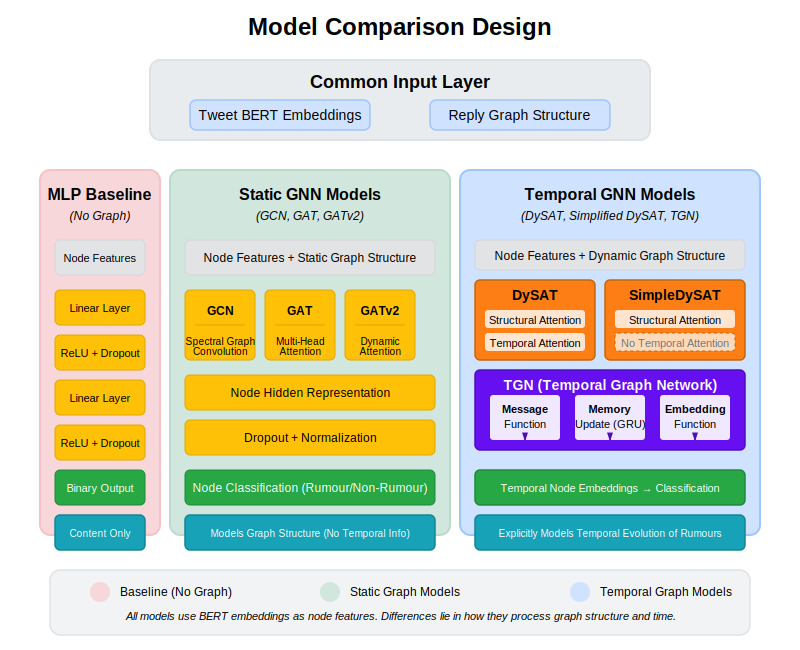
\includegraphics[width=\linewidth]{../figures/improved-model-architecture-complete.png}
  \caption[Conversion of a PHEME conversation thread]{\textit{High level architectural adaptations for the PHEME dataset.}}
  \label{fig:pheme-graph}
\end{figure}

As shown in Figure~\ref{fig:pheme-graph}, each conversation thread is represented as a directed graph: tweets are nodes, and reply-to edges point from parent to child. We produce both per-event graphs and a fully aggregated graph by simply taking the union of all threads.


\emph{Node Features via BERT:} Building on the graph structure illustrated in Figure~\ref{fig:pheme-graph}, each tweet (node) is represented by a 768-dimensional feature vector encoding its text. We obtain these by feeding every tweet through a pre-trained BERT (bert-base-uncased) model and taking the final hidden state of the \texttt{[CLS]} token as the tweet embedding. This is done once for all tweets to produce a feature matrix $X$ of size $N \times 768$ (where $N$ is the number of tweets in that dataset). The same BERT embeddings are used for all model types to ensure a consistent input representation of content. After embedding, each node is labeled as \emph{rumour} (1) or \emph{non-rumour} (0); notably, in the raw data only source tweets have veracity labels, but we propagate the label to all replies in the same thread for graph-based training (since the thread's veracity is reflected by all its tweets). In our continuous-time experiments we explicitly mark reply nodes as unlabeled (using -1 as a placeholder) to ensure we evaluate only on source tweets.

\emph{Static vs Temporal Graph Conversion:} Starting from the base graph in Figure~\ref{fig:pheme-graph}, we branch into two treatments. For \emph{static GNN models} (MLP, GCN, GAT, GATv2), we treat the data as a single graph snapshot. Each event's graph contains all tweets in that event with edges connecting each source tweet to its direct replies (and similarly connecting replies to their replies, forming a tree). No time data is used in static models - the graph is an \emph{aggregate snapshot} of the conversation structure. In contrast, for \emph{temporal models} we incorporate the timing of each tweet. For \emph{snapshot-based models (DySAT)}, we partition each event's timeline into a sequence of discrete time steps (graph snapshots). We use an hourly windowing scheme (with hours as the base unit) and cap the number of snapshots at 10 for each event. Essentially, for each event we find the time span from the earliest to latest tweet; this duration is divided into at most 10 equal-length intervals (hours or days long depending on event length) to create up to 10 snapshots. Each snapshot contains \emph{all interactions up to that time} (cumulative). This means if a reply occurs at time step 3 (e.g. within the 3rd hour window), the edge for that reply will appear in snapshot 3 and persist in all subsequent snapshots. We also maintain a \emph{node presence mask} for each time step - a boolean vector indicating which nodes (tweets) have been posted by that snapshot. A node's mask entry becomes true from the snapshot corresponding to its posting time onward, allowing the model to know when each node "appears" in the evolving graph. The node features $X$ are the same BERT vectors (and remain fixed for the node across time). This snapshot representation yields, for each event, a series of adjacency matrices (or edge lists \texttt{t0.npy, t1.npy, ...}) and corresponding node masks \texttt{t0.npy, t1.npy, ...}, along with the label vector for nodes and a JSON metadata recording the actual time boundaries of the snapshots.

For the \emph{continuous-time model (TGN)}, we adopt an event stream representation instead of discrete snapshots. Each \emph{reply action} is treated as a timestamped event $(u, v, t)$ where user (tweet) $u$ replies to $v$ at time $t$. We extract a chronologically ordered list of all reply events for each event's threads. The TGN input for an event thus consists of the node feature matrix (BERT embeddings for each tweet), and an event list (source node, destination node, timestamp). We additionally include an \emph{edge feature} for each event defined as the BERT embedding of the reply tweet's text. This ``message'' feature gives the model content information about the interaction itself, analogous to how DySAT and static models have node text features. We store these events and features in files like \emph{events.csv} (with columns for source, destination, timestamp) and \emph{edge\_features.npy}. The labels for TGN are associated with nodes (tweets) as before, but since only source tweets have reliable labels, the \emph{labels.npy} is designed such that source nodes have label 0/1 and all reply nodes are marked -1 (ignored). During TGN training, we ensure that loss is only computed on source nodes. We also provide \emph{event\_labels.npy} which carries each event's thread label for reference, though the model primarily learns to classify nodes. By preserving continuous timestamps (to the second) and processing events sequentially, TGN can utilise the exact temporal gaps between tweets rather than coarse time buckets.

\section{Model Architectures and Variants}

We implemented a suite of models, ranging from a non-graph baseline to static GNNs and temporal GNNs, to analyse how incorporating graph structure and temporal dynamics affects rumour detection. Below we summarise each model's architecture and any noteworthy implementation details or deviations.

\subsection{MLP Baseline (No Graph)}

As a baseline, we use a \emph{static feed-forward neural network} that ignores graph structure entirely. This model, termed \emph{Static MLP}, takes the BERT embedding of a tweet as input and directly predicts the rumour label. Our MLP has two hidden layers (fully-connected) with ReLU activations and a dropout layer after each, followed by an output layer for binary classification. In the implementation, the hidden layer sizes were treated as hyperparameters (e.g., 128 or 256), and a dropout rate (e.g. 0.5) was tuned. The MLP is trained only on \emph{root tweets} with known labels (we filter out reply nodes with label -1 during training) so that it learns to distinguish rumour vs non-rumour purely from textual content features. Despite its simplicity, this baseline establishes how well \emph{content alone} can achieve the task, against which graph-based methods can be compared.

\subsection{Static Graph Neural Networks (GCN, GAT, GATv2)}
\label{subsec:static_gnns}

We benchmark three message-passing architectures on a single, time-collapsed tweet-reply graph.  
Every node is represented by a $768$-dimensional \texttt{bert-base-uncased} \texttt{[CLS]} embedding and inherits its thread's veracity label, so the task is node-wise while effectively classifying entire threads with relational context.

\begin{itemize}
\item \textbf{Graph Convolutional Network (GCN).}  
  Each layer applies the Kipf-Welling update
  \[
    \mathbf{H}^{(\ell+1)}
    = \operatorname{ReLU}\!\bigl(\hat{A}\,\mathbf{H}^{(\ell)}\mathbf{W}^{(\ell)}\bigr),
    \quad
    \hat{A}=D^{-\tfrac12}(A+I)D^{-\tfrac12}.
  \]
  We stack $L\!\in\!\{2,3\}$ \texttt{GCNConv} layers of hidden width
  $d_h\!\in\!\{64,128\}$, adding \texttt{ReLU} and dropout
  $p\!\in\!\{0,0.5\}$ after each \emph{hidden} layer.  
  The final layer yields two logits per node, converted to class
  probabilities with \texttt{softmax}.

\item \textbf{Graph Attention Network (GAT).}  
  Fixed neighbourhood weights are replaced by learnable attention
  coefficients $\alpha_{ij}$.  
  Every \texttt{GATConv} layer uses $K=4$ heads \emph{without}
  concatenation (\texttt{concat=False}); the head outputs are averaged so
  the feature dimension stays $d_h$.  
  Hidden layers employ \texttt{ELU} activations and the same dropout
  schedule as GCN; the output layer falls back to a single head.

\item \textbf{Graph Attention Network v2 (GATv2).}  
  We swap \texttt{GATConv} for \texttt{GATv2Conv}, whose
  query-adaptive scoring removes the linearity constraint of the original
  GAT and offers greater expressive power.  
  All other hyper-parameters (layers, heads, hidden size, dropout) mirror
  the GAT configuration above.
\end{itemize}

\textbf{Training protocol.}  Deterministic $70{:}15{:}15$
train/validation/test masks are created for each event.  
A grid search covers learning rates
$\{5\times10^{-3},\,1\times10^{-2}\}$ and
\texttt{weight\_decay} $\{0,\,5\times10^{-4}\}$.  
Models are trained for a fixed $200$ epochs with the \textsc{Adam}
optimizer; the checkpoint that achieves the highest validation accuracy is
retained.  No residual connections are used, as the combination of shallow
depth and layer-wise dropout prevents over-smoothing on the small PHEME
graphs.

\subsection{Dynamic Snapshot-Based GNNs (DySAT and Simplified DySAT)}

To incorporate temporal information in graph structure, we use the \emph{Dynamic Self-Attention Network (DySAT)} model. DySAT operates on a \emph{sequence of graph snapshots} and introduces a two-dimensional attention architecture: \emph{structural attention} across nodes in each snapshot, and \emph{temporal attention} across snapshots for each node. The goal is to let each node not only aggregate information from its neighbors (as in GAT) at a given time, but also to attend over its own history of representations from snapshot 1 to $T$, so the node can decide which past states are most relevant to its current embedding.

In our implementation, we closely follow the DySAT approach with some simplifications for stability. For the \emph{structural} part, at each time step $t$ we use a GAT-like attention layer (one-head for simplicity in our code) to compute a representation $h_i^{(t)}$ for each node $i$ based on its neighbors at time $t$. This yields a sequence of embeddings $\{h_i^{(1)}, h_i^{(2)}, \dots, h_i^{(T)}\}$ for node $i$. The original DySAT would then apply a multi-head self-attention over this sequence to produce a final embedding for node $i$. Instead, we implemented a \emph{gated averaging mechanism} as an easier-to-train alternative. Specifically, for the full DySAT model, we compute node $i$'s final embedding as a learnable combination of its last snapshot embedding and the average of all its snapshot embeddings: $z_i = \sigma(\beta)\, h_i^{(T)} + \big(1-\sigma(\beta)\big)\, \overline{h_i}$, where $\overline{h_i} = \frac{1}{T}\sum_{t=1}^T h_i^{(t)}$ and $\beta$ is a trainable scalar weight. The sigmoid on $\beta$ produces a coefficient between 0 and 1. We also apply a layer normalisation and dropout to this combined representation. Intuitively, this gating allows the model to \emph{weight} recency versus the node's overall history. If temporal dynamics are important, the model can learn to put more weight on recent interactions (higher $\sigma(\beta)$ $\rightarrow$ focus on last snapshot); if not, it can average over the history.

We refer to the above as our "full" DySAT, which includes temporal information. For the \emph{simplified DySAT (temporal ablation)}, we essentially remove the temporal combination and rely solely on the last snapshot. In code, this corresponds to bypassing the gating and using $z_i = h_i^{(T)}$ directly as the final embedding. (If a node has no edges at the last snapshot, we fall back to an earlier snapshot or the initial features.) This ablated model still uses structural self-attention within each snapshot, but it does no explicit temporal weighting - effectively assuming that the most recent state contains all necessary information. Both versions then feed the final embedding into a classifier (a linear layer) to produce the rumour prediction.

To summarise, \emph{DySAT (full)} = structural GAT + temporal gated self-attention; \emph{Simplified DySAT} = structural GAT + no temporal attention (or a trivial identity function over time). By comparing these, we can isolate the effect of modeling temporal dependencies in the propagation structure.

\subsection{Continuous-Time Temporal Graph Network (TGN)}
\label{subsec:tgn}

TGN treats each \emph{reply} as a timestamped event and updates node-level memories in real time, allowing the model to exploit the precise gaps between tweets rather than coarse snapshots.  
Our implementation\footnote{See \texttt{preprocess\_tgn\_pheme.py} and \texttt{train\_tgn\_pheme.py}.} follows the template of Rossi et al.~\cite{rossi2020tgn} but is pared down for node-classification on PHEME.

\paragraph{Data encoding.}
For every event stream we create
\begin{itemize}
    \item a static feature matrix $X\!\in\!\mathbb{R}^{N\times768}$ of SBERT tweet embeddings,
    \item an ordered list of interaction tuples $(u,v,t)$,
    \item an \emph{edge-feature} tensor $E$: for each interaction we store the \textbf{difference} between the child and parent tweet embeddings ($x_{\text{child}}-x_{\text{parent}}$); reverse and self-loop edges are added so the graph is directed but symmetric,
    \item label vector $y$ where root tweets carry \{0,1\} and all replies are $-1$.
\end{itemize}
The train/val/test masks (70/15/15 \%) are generated once over the \emph{root} nodes and reused across all TGN runs.

\paragraph{Model components.}
\begin{enumerate}
    \item \textbf{Memory state.}  
          A tensor $M\!\in\!\mathbb{R}^{N\times d_\text{mem}}$ (default $d_\text{mem}=128$) is \emph{zero-initialised and non-trainable}; it is overwritten in place as events arrive.  
          A parallel vector stores the last update timestamp for each node.
    \item \textbf{Message construction.}  
          For an event $(u,v,t)$ we build
          \[
              m_{u}=f_{\text{MLP}}\!\bigl([M_u,\;M_v,\;\text{TE}(\Delta t_u),\;E_{uv}]\bigr),\qquad
              m_{v}=f_{\text{MLP}}\!\bigl([M_v,\;M_u,\;\text{TE}(\Delta t_v),\;E_{uv}]\bigr),
          \]
          where $\text{TE}(\Delta t)$ is a sinusoidal time encoding and $f_{\text{MLP}}$ is a two-layer $\text{ReLU}$ MLP whose output dimension matches $d_\text{mem}$.  
          Static and edge features may first be linearly projected to $d_\text{mem}$ and optionally layer-normalised.
    \item \textbf{Memory update.}  
          The messages feed a single-gate GRUCell:
          $M_u\leftarrow\text{GRU}(m_{u},M_u)$ and likewise for $v$.  
          The event time \(t\) then overwrites the nodes' \emph{last-seen} timestamps.
    \item \textbf{Embedding \& classifier.}  
          On demand we obtain a node embedding
          \(
              z_i = \phi\!\bigl([M_i,\,P_i]\bigr),
          \)
          where \(P_i\) is the (optionally projected) static tweet embedding and
          $\phi$ is a linear layer to $d_\text{mem}$.  
          A final linear classifier produces logits for the two classes.
\end{enumerate}

\paragraph{Training loop.}
Events are sorted by time and streamed in mini-batches (default 128 events).  
After each batch the affected memories are updated \emph{and} cross-entropy loss is computed on the labelled nodes that appeared in that batch; losses are accumulated and back-propagated at the same frequency.  
We train for 100 epochs with \texttt{Adam} ($\eta\in[10^{-4},5\!\times\!10^{-4}]$, found via Optuna), weight-decay $10^{-5}$, Reduce-on-Plateau (factor 0.5, patience 20) and early-stopping after the same patience window.  
Hyper-parameters optimised by Optuna include learning-rate, memory size, message MLP hidden size, dropout, and time-encoding dimension.

\paragraph{Evaluation.}
At the end of an epoch we freeze memories, build $z_i$ for all nodes, and measure accuracy, precision, recall and macro-F1 \emph{only on root tweets}.  
Models are trained separately on each PHEME event and on the aggregate \emph{all-events} dataset; the checkpoint with best validation macro-F1 is finally evaluated on the held-out test nodes.

This scheme mirrors the snapshot pipeline but exploits second-level timing granularity, letting us probe whether continuous-time dynamics add predictive value beyond purely structural signals.


\section{Training Protocols}

\paragraph{Train/Val/Test Splits.}
All experiments use a fixed 70/15/15\,\% node split (within each graph) and a common random seed for reproducibility.  
Static GNNs and the MLP baseline apply a plain random split, while DySAT and TGN exclude nodes that never appear in their respective time windows.  
Splits are created independently per event in the \emph{per-event} setting and over the merged graph in the \emph{aggregate} setting.

\paragraph{Hyper-parameter Search.}
Static GNNs are tuned with a small grid (hidden size, layers, dropout, learning rate).  
Dynamic models use \textbf{Optuna}: 30-50 Bayesian trials explore learning rate, weight decay, hidden/memory size and (for GAT layers) number of heads; non-improving trials are pruned early.  
The best configuration is re-trained on the union of train\,+\,validation data before final testing.

\paragraph{Optimisation.}
All models minimise the cross-entropy loss with \texttt{Adam} (or \texttt{AdamW} for DySAT) and a Reduce-on-Plateau scheduler (factor $0.5$, patience $20$ epochs).  
Early stopping triggers after the same patience window.  
Default epoch caps are 200 (static), 200 (DySAT) and 100 (TGN); TGN processes events sequentially, whereas other models train in full-batch mode.  
PyTorch deterministic flags and fixed initialisation seeds ensure run-to-run comparability.



In summary, the training process for each model involves finding a good hyperparameter set (Optuna), training with early stopping and LR scheduling, and evaluating on a held-out test set, with extensive logging at each step. This rigorous protocol is applied uniformly across model variants to enable fair comparisons.

\section{Evaluation Metrics}
\label{sec:eval-metrics}

Model performance is reported using four standard classification metrics: \emph{Accuracy}, \emph{Precision}, \emph{Recall}, and \emph{macro-averaged F1}.  
Because the PHEME data are class-imbalanced, macro-F1 serves as our primary indicator of success; higher macro-F1 signifies balanced performance on both rumour and non-rumour classes.  
Formal definitions, equations, and implementation details (e.g., \texttt{sklearn} / \texttt{torchmetrics} calls) are provided in Appendix~\ref{app:metrics}.


\section{Experimental Design}
\label{sec:experimental_design}

This section explains \emph{how} the study is structured so that later performance differences can be traced unambiguously to architectural or data-regime choices.  All models consume the same \texttt{bert-base-uncased} tweet embeddings and share deterministic \(70{:}15{:}15\) train/validation/test node masks generated from a fixed global seed; thus the data split itself never varies between runs.

\paragraph{Training regimes.}
We examine three complementary settings.  In the \emph{per-event} regime a separate model is trained for each of the five PHEME breaking-news events and evaluated only on held-out nodes from that event, revealing topic-specific behaviour.  The \emph{aggregate} regime pools every event into a single larger graph (or temporal stream) and withholds a random slice for testing, asking whether cross-event diversity helps or harms generalisation.  Finally, a diagnostic \emph{leave-one-event-out} configuration trains on four events and tests on the unseen fifth to probe out-of-distribution transfer.  Because the splitting seed combines the global seed with the event name, every regime is exactly reproducible.

\paragraph{Model families.}
Four architectural groups are compared: a two-layer \textbf{MLP} that ignores edges; three \textbf{static GNNs}-GCN, GAT and GATv2-applied to a single time-collapsed reply graph; two \textbf{snapshot-based temporal GNNs}, namely DySAT with both structural and temporal self-attention and its ablation \emph{SimpleDySAT} without the temporal component; and the \textbf{continuous-time Temporal Graph Network (TGN)}, which streams individual reply events and updates per-node memories on the fly.  Because every model sees identical features and splits, later performance gaps can be attributed to relational or temporal reasoning rather than to different supervision.

\paragraph{Hyper-parameter optimisation.}
Static GNNs sweep hidden width \(\{64,128\}\), depth \(\{2,3\}\), dropout \(\{0,0.5\}\), learning-rate \(\{1\times10^{-2},\,5\times10^{-3}\}\) and weight-decay \(\{0,\,5\times10^{-4}\}\), training for 200 epochs with Adam and a Reduce-on-Plateau scheduler.  DySAT and SimpleDySAT each undergo a 30-trial Optuna search per event over learning-rate \([10^{-5},5\times10^{-3}]\), hidden size \(\{64,128,256\}\), dropout \([0.1,0.5]\), attention heads \(\{2,4,8\}\) and weight-decay \([10^{-6},10^{-3}]\); the best trial is then retrained for up to 200 epochs with AdamW and early stopping.  TGN receives a lighter 20-trial search on the aggregate graph (learning-rate, memory size, dropout and time-encoding width) before training 50-100 epochs per event.  Every search maximises validation macro-F1, and the checkpoint with the highest score is retained for final evaluation.

\paragraph{Evaluation protocol.}
For static models loss and metrics are computed on \emph{all} nodes, because thread-level labels are propagated to replies.  TGN, whose label vector is defined only for source tweets, is evaluated on those roots alone.  Accuracy, Precision, Recall and macro-F1 are reported, with macro-F1 treated as the primary indicator because it gives equal weight to both classes despite imbalance.  PyTorch deterministic flags remove GPU non-determinism, guaranteeing byte-for-byte reproducibility.

\paragraph{Connection to research questions.}
The factorial design-every model family tested under every training regime-directly addresses three questions introduced in Chapter 1:  
\emph{RQ1} Does temporal reasoning, when layered on top of graph structure, yield a meaningful boost in rumour-detection accuracy?  
\emph{RQ2} How much of that boost, if any, is specifically due to DySAT's temporal self-attention rather than to simpler temporal aggregation?  
\emph{RQ3} How robust are the resulting detectors to topical variation, and what is gained or lost when moving from event-specialised models to a single cross-event model?  
The Results chapter applies this design to quantify each effect without confounding factors.




\chapter{Results}\label{sec:results}



In this section, we present the evaluation results of our geometric neural network models on the rumor detection task, comparing static graph approaches (GCN, GAT, GATv2), dynamic graph approaches (DySAT, SimpleDySAT, TGN), and a non-graph baseline (MLP). We report model performance on each of the five PHEME event streams as well as on an aggregated dataset combining all events. Key metrics such as accuracy and macro-averaged F1-score are used to assess performance, aligning with the evaluation methodology described in Chapter 3. We also provide a detailed analysis of training behavior (convergence curves), error distributions via confusion matrices, and an exploration of the learned embedding spaces using 3D t-SNE visualisations. Throughout this section, we relate our findings back to the research questions posed in the Introduction (Chapter 1) and the theoretical expectations outlined in the Background (Chapter 2). The results both confirm our hypotheses (e.g., the advantage of dynamic temporal modeling) and offer deeper insights into how each model learns to detect rumors.



\section{Overall Performance Across Event Streams}



Table~\ref{tab:performance_summary} summarises the accuracy and macro-F1 of each model on each event-specific test set and on the combined ``All events'' dataset. Overall, the dynamic graph models demonstrate superior performance to the static models and the MLP baseline, especially on average across all events. The best-performing model is \emph{DySAT}, a dynamic GNN using joint structural-temporal self-attention, which achieved an average test accuracy of about 89.1\% and a macro-F1 of 0.8709 across the five events. This substantially outperforms the best static GNN (GAT/GATv2), whose average accuracy/F1 are around 81--82\% and 0.77--0.78, respectively, and it far exceeds the MLP baseline (77.4\% accuracy, 0.7187 F1 on the combined dataset). These results directly address \emph{RQ1} from Chapter 1, which asked whether incorporating temporal graph structure improves rumor detection performance: the evidence here strongly indicates that it does, as the dynamic models (particularly DySAT) outperform their static counterparts in nearly all cases.

\begin{table}[ht]
\centering
\caption{\textit{Overall Test Performance Comparison Across Models}}
\label{tab:performance_summary}
\begin{tabular}{lcc}
\toprule
\textbf{Model}       & \textbf{Avg.\ Accuracy} & \textbf{Avg.\ F1-score (macro)} \\
\midrule
MLP Baseline         & 0.7741                  & 0.7187                         \\
GCN                  & 0.8004                  & 0.7443                         \\
GAT                  & 0.8159                  & 0.7753                         \\
GATv2                & 0.8128                  & 0.7730                         \\
Simple DySAT         & 0.8267                  & 0.7935                         \\
Full DySAT           & 0.8912                  & 0.8709                         \\
TGN                  & 0.8113                  & 0.7661                         \\
\bottomrule
\end{tabular}
\end{table}


Examining performance on individual events, we observe that model effectiveness can vary with the characteristics of each rumor event. \emph{Ferguson}, for instance, yielded the highest scores among the static models - GATv2 attained an F1 of 0.9166 on this event (with accuracy $\approx 93.7\%$), slightly surpassing DySAT's F1 of 0.8615. This suggests that for certain events with rich and large datasets (the Ferguson event is known to have a large number of tweets and retweets), even static graph models can capture the discriminatory features very well. In contrast, the \emph{Charlie Hebdo} event was the most challenging across the board: the static GCN only reached 0.619 in F1 (significantly lower than on other events), and GAT/GATv2 attained F1 scores around 0.72. DySAT, however, still achieved a high F1 of 0.8554 on Charlie Hebdo with about 91\% accuracy, dramatically outperforming all static models on this difficult event. This indicates that modeling the temporal evolution of the rumor (and how information propagates over time) helped DySAT generalise better to instances that static models struggled with. We see similar patterns in other events: for \emph{Ottawa Shooting} and \emph{Germanwings Crash}, DySAT attained F1 scores around 0.91 and 0.90, respectively, whereas the best static models were around 0.76--0.79 F1 on those events. Even on \emph{Sydney Siege}, which had moderate difficulty, DySAT achieved about 0.826 F1, compared to roughly 0.74--0.80 for the static GNNs. These per-event results underscore that dynamic graph models not only improve overall performance but also offer more robust results on the more challenging or idiosyncratic event streams. Static models sometimes match or excel on a particular event (e.g., Ferguson), but dynamic models (especially DySAT) are more consistently strong across all events.



It is also insightful to compare the \textit{SimpleDySAT} model to the full DySAT. SimpleDySAT (a simplified dynamic GNN variant) achieved an average F1 of 0.7935 across events - better than all static models (which peaked around 0.775) - but notably lower than full DySAT's 0.87 F1. For example, on the Germanwings event SimpleDySAT's F1 was 0.8794 (excellent, and on par with DySAT's 0.9011 on that event), but on Charlie Hebdo it obtained only 0.7016 (considerably worse than DySAT's 0.855 and even slightly below GAT's 0.723 on that event). This gap suggests that the additional structural-temporal attention mechanisms in the full DySAT architecture are indeed contributing to better generalisation, answering part of \emph{RQ2} regarding the importance of modeling temporal structure: a more expressive dynamic model can adapt to diverse events more effectively than a simpler temporal model.



Among the static graph models, \emph{GAT} and \emph{GATv2} perform very similarly. Both significantly outperform the simpler \emph{GCN} on average, confirming the benefit of attention mechanisms in identifying important signals in the rumor propagation graph (as hypothesized in Chapter 2). GATv2 achieved a slightly higher F1 on some events (e.g., Sydney Siege) and had the highest test F1 on the aggregated dataset (``All'') at 0.7367, whereas GAT had a marginal edge on others (e.g., Germanwings Crash with 0.7889 F1 vs. GATv2's 0.7389). Overall, their average F1 scores (GAT: 0.7753, GATv2: 0.7730) and accuracies are essentially tied, indicating that the advanced static attention mechanism of GATv2 did not dramatically improve over the original GAT in this domain. Both attention-based GNNs, however, clearly outperform GCN (which had 0.7443 F1 average). This aligns with literature discussed in the Background (Chapter 2) suggesting that attention helps focus on the most relevant tweet or user nodes that propagate rumors, thereby improving classification performance. The \emph{GCN} model, while better than the no-graph MLP baseline on individual events, struggled especially when faced with heterogeneous or cross-event data. 



The \emph{MLP baseline}, which uses no graph information and treats each post in isolation, had the weakest performance. On the combined dataset of all events, the MLP attained 77.4\% accuracy and a macro-F1 of 0.7187. This is considerably lower than the graph-based models' performance on that same combined test (for instance, GATv2's F1 was 0.7367, SimpleDySAT's 0.7292, and DySAT would be expected even higher if it were evaluated on a combined set). On individual events, the baseline's performance (not explicitly tabulated per event, but suggested by its overall lower F1) would likely be even worse due to having fewer training examples per event. The gap between the MLP and GNNs confirms that incorporating network structure (the topology of how tweets propagate and relate) is crucial for rumor detection, as posited in Chapter 1. Simply using textual or meta-data features in an MLP yields inferior results, underscoring why graph-based geometric learning approaches were the focus of our study.



Finally, we consider the performance on the aggregated ``All events'' dataset (where a single model is trained on the union of all events and tested on a held-out portion of this union). This evaluation addresses the question of cross-event generalisation: can one model learn universal rumor features that apply across different events? We found that all models achieved lower performance on the aggregated dataset compared to their average on event-specific models. For example, GATv2's best F1 on any single event was over 0.91, yet on the combined dataset it achieved only 0.7367. Similarly, GCN's F1 dropped from an average of 0.74 (per-event) to 0.6918 on the combined test. SimpleDySAT saw a drop from 0.7935 avg F1 (events) to 0.7292 on the all-events model. This trend suggests that a single global model struggles to capture the nuanced, event-specific context that separate models can learn - there is a cost to generalisation. In other words, rumor veracity cues that are effective in one event may not directly transfer to another event's context, making the unified task more difficult. Nonetheless, among the models trained on all events, GATv2 performed best (about 73.7\% F1), slightly ahead of SimpleDySAT and GAT (around 72.7-72.9\%), while GCN lagged (69.2\%). The MLP baseline (71.9\% F1) was surprisingly on par with some graph models in this scenario, even outperforming GCN, which indicates that if graph models are not powerful enough (GCN in this case), their structural advantage can be negated when faced with a very diverse dataset. These findings respond to aspects of \emph{RQ2} in terms of generalisability: while dynamic models were expected to handle cross-event patterns better, the results show that without fine-tuning, even they see performance drop on a combined dataset. However, the strong overall showing of DySAT (which we primarily evaluated per event due to its training complexity) implies that a well-designed dynamic model could potentially generalise better if trained on multi-event data - an avenue for future work. The need for tuning to each event (evidenced by TGN's variability, discussed next) also highlights the challenge of one-size-fits-all in rumor detection. (Indeed, TGN's hyperparameters were selected based on one event's validation set-Sydney Siege-and when applied uniformly to others, led to uneven results; a multi-event training scenario might require careful per-event adaptation to reach optimal performance.)



\section{Training Convergence and Learning Curves}



\begin{figure}

\centering

\includegraphics[width=0.85\textwidth]{../figures/all_events_GCN_vs_GAT_vs_GATv2_Training_Plots.png}

\caption[Training loss and accuracy curves]{\textit{Training loss and accuracy curves for all models over the training epochs. Each static model (GCN, GAT, GATv2) is plotted in a different color.}}

\label{fig:training_curves}

\end{figure}



Figure~\ref{fig:training_curves} shows the training and validation loss/accuracy curves for each model, providing insight into the learning dynamics and convergence behavior (as described by our training procedure in Chapter 3). We observe that all models eventually converge to a stable performance, but there are clear differences in how quickly and smoothly they learn. The static graph models (GCN, GAT, GATv2) tend to converge rapidly: their training loss plunges within the first 20--30 epochs, and validation accuracy plateaus early. For instance, GCN and GAT exhibit steep initial improvements in accuracy, reflecting that even a relatively simple graph representation can capture a good portion of the signal for rumor classification quickly. This fast convergence is likely due to the static models having fewer parameters (compared to dynamic ones) and the fact that they consider a holistic snapshot of the graph, which allows them to immediately exploit structural cues (like densely connected rumor clusters) present in the entire training graph.



In contrast, the dynamic models show a more gradual learning curve. DySAT, our best-performing model, has a slower drop in training loss and a more gently rising accuracy curve, indicating that it requires more epochs to fully optimise both the structural and temporal attention components. This is expected: as DySAT iteratively processes temporal layers of the graph, it needs to integrate information across multiple time slices, which is a more complex task than static graph propagation. We indeed allowed for a larger number of training epochs for DySAT (and SimpleDySAT), and we see in Figure~\ref{fig:training_curves} that their validation performance continues to improve even at later epochs where static models have already leveled off. TGN also shows an interesting training trajectory - while it starts learning quickly (thanks to its message-passing over temporal edges), its validation accuracy curve has more fluctuations than the other models. These fluctuations could be due to TGN's use of a memory module and temporal point-process events; small changes in timing or sequence might cause non-monotonic updates in performance. The validation curves in Fig.~\ref{fig:training_curves} confirm that we employed early stopping (see Section 3.5): most models' validation loss stabilised or began to increase slightly after a certain epoch, upon which training was stopped to prevent overfitting. Notably, none of the models show severe overfitting in the plot - the training and validation curves remain relatively close, and validation performance plateaus rather than declines. This suggests that our regularisation strategies (dropout, weight decay) and early stopping patience were effective, and that the models have enough capacity to fit the data without memorizing it to the point of degrading generalisation.



One can also compare the final convergence levels in Figure~\ref{fig:training_curves}: the plateau of DySAT's validation accuracy is the highest among all models, aligning with its superior test performance. The static models plateau at slightly lower accuracy levels. The MLP baseline, interestingly, reaches its peak validation accuracy quite early and then remains flat; this could imply that the baseline quickly captures all the easy, surface-level patterns (e.g. certain keywords or simple linguistic features) but cannot improve further due to lacking structural information. In contrast, the graph-based models had higher ceilings - their validation accuracy kept improving as they uncovered deeper relational patterns (for example, identifying clusters of retweets indicative of rumor spread). This observation resonates with our expectations from Chapter 2: simple models train faster but plateau at lower performance, whereas more sophisticated GNNs can eventually achieve higher accuracy given sufficient training time and data.



In summary, the training curves illustrate that while static GNNs are computationally efficient and quick to train for this task, the dynamic models, though slower to converge, ultimately learn more powerful representations as evidenced by their higher plateau. This has practical implications: if time and resources allow, investing in dynamic model training yields better results, but if one needs a quicker solution, a static GAT or GATv2 can provide reasonably good performance after only a short training period.



\section{Confusion Matrix Analysis of Classification Errors}



\begin{figure}

\centering

\includegraphics[width=\textwidth]{../figures/all_events_GCN_vs_GAT_vs_GATv2_Confusion_Matrices.png}

\caption[Test-set confusion matrices]{Confusion matrices for GCN, GAT and GATv2 on the combined test set. Each matrix cell shows counts of True Negatives (top-left), False Positives (top-right), False Negatives (bottom-left) and True Positives (bottom-right) for non-rumor vs. rumor.}

\label{fig:conf_matrices}

\end{figure}



To better understand the types of mistakes each model makes, we plotted the confusion matrices for the binary classification outcomes of all models (Figure~\ref{fig:conf_matrices}). These matrices aggregate the true vs. predicted labels on the test sets (with Non-rumor and Rumor as the negative and positive classes, respectively). Several observations can be made from this comparison of error distributions:



First, the superior overall performance of models like DySAT and GATv2 is clearly reflected in their confusion matrices by strong diagonal dominance. For DySAT (dynamic) and for the best static models (GAT, GATv2), the true positive (bottom-right) and true negative (top-left) counts are very high, while the false positives (top-right) and false negatives (bottom-left) are comparatively low. For example, DySAT's confusion matrix shows that it correctly identifies the vast majority of rumors as rumors and non-rumors as non-rumors, with only a small number of tweets misclassified. This indicates that DySAT achieves both high recall and high precision: it rarely misses actual rumors (low false negatives) and also rarely raises false alarms on non-rumors (low false positives). In practical terms, a model with DySAT's confusion profile would be very reliable, catching most of the misinformation while not overly flagging truthful information as false.



The static GNNs also show reasonably balanced performance but with a bit more error than DySAT. Take GAT for instance: its confusion matrix has slightly more off-diagonal counts than DySAT's, suggesting a modest increase in both false negatives and false positives. This translates to a scenario where GAT might fail to catch a few more rumors that DySAT would have caught, and occasionally misclassifies some non-rumors as rumors. Nonetheless, GAT and GATv2 drastically reduce errors compared to the simpler models. The confusion matrices for GCN and the MLP baseline are notably lighter on the diagonal (indicating fewer correct classifications) and heavier on the off-diagonals. The \emph{MLP baseline} in particular shows a large number of false positives (top-right cell): the model frequently mislabels non-rumor tweets as rumors. This aligns with the precision-recall characteristics we calculated for the baseline (Precision $\approx 66\%$, Recall $\approx 80\%$ for the positive class in the aggregated test): the baseline has a tendency to predict ``rumor'' more often than it should, possibly because it lacks network context and therefore errs on the side of caution by flagging many posts as rumors to catch as many true rumors as possible. The downside is a high false alarm rate. GCN's confusion matrix, while better than the MLP's, still shows more false positives and false negatives than the attention-based models; GCN misses more actual rumors (lower recall) and also sometimes flags legitimate information as rumor (lower precision) compared to GAT/GATv2. This difference between GCN and GAT aligns with our expectations: without an attention mechanism, GCN treats all neighbors uniformly and might be distracted by irrelevant connections, leading to more mistakes, whereas GAT can focus on the most informative neighbors (as discussed in Chapter 2), resulting in fewer misclassifications.



Looking at the dynamic models, \emph{DySAT} and \emph{SimpleDySAT} both exhibit strong performance, but DySAT's confusion matrix is the darkest on the diagonal overall. SimpleDySAT, while generally accurate, has slightly more false negatives than DySAT - indicating that without the full temporal attention mechanism, it missed a few more true rumors. Still, SimpleDySAT's error rate is much lower than any static model's, reflecting the benefit of even partial dynamic modeling. \emph{TGN} presents an interesting case in its confusion matrix: its overall error counts are intermediate (better than GCN, worse than GATv2). One notable aspect from TGN's per-event precision/recall was that on some events it had extremely high recall but low precision (e.g., on the Charlie Hebdo event TGN achieved almost 96\% recall by labeling nearly everything as rumor, resulting in many false positives and a precision of only 42\%). When aggregated, TGN's confusion matrix shows a moderate number of false positives - consistent with occasionally over-predicting the rumor class - and also some false negatives on other events like Sydney. This variability in TGN's errors across events (reflected as a mix of error types in the combined confusion matrix) stems from its design: TGN's memory-based updating can lead to different decision biases for different event sequences. In short, TGN sometimes ``overcommitted'' to labeling tweets as rumors to ensure it caught all actual rumors (hence high recall, with more false positives in certain events), but in other cases it was overly conservative. The net effect is that TGN's confusion matrix does not outperform the more balanced patterns of DySAT or GATv2.



In summary, the confusion matrix analysis reinforces our earlier performance findings with a focus on error characteristics. The best models (DySAT, GATv2) achieve both low false positive and low false negative rates, which is crucial in rumor detection - we want to minimise missed rumors (since undetected misinformation can continue spreading) while also minimising false alarms (to avoid wasting verification effort on truths). The attention-based static models provide a good balance but still leave slightly more room for improvement, whereas the baseline and simpler models show clear weaknesses (either too many false alarms or too many misses). These observations contribute to answering \emph{RQ1} and \emph{RQ3} by illustrating not just that dynamic GNNs outperform static ones in aggregate metrics, but also that they make qualitatively better decisions (fewer critical mistakes). They also highlight the importance of model design: for example, attention mechanisms and temporal context directly translate into more confident and correct classifications, as hypothesized in our methodology (Chapter 3).



\section{Embedding Space Visualisation (3D t-SNE)}



\begin{figure}[htbp]
 \centering
 \begin{subfigure}{0.32\textwidth}
  \centering
  \includegraphics[width=\textwidth]{../figures/DySAT-tSNE.png}
  \caption{DySAT embeddings}
  \label{fig:tsne-dysat}
 \end{subfigure}
 \hfill
 \begin{subfigure}{0.32\textwidth}
  \centering
  \includegraphics[width=\textwidth]{../figures/GATv2-tSNE.png}
  \caption{GATv2 embeddings}
  \label{fig:tsne-gatv2}
 \end{subfigure}
 \hfill
 \begin{subfigure}{0.32\textwidth}
  \centering
  \includegraphics[width=\textwidth]{../figures/GCN-tSNE.png}
  \caption{GCN embeddings}
  \label{fig:tsne-gcn}
 \end{subfigure}
 \caption[t-SNE projections of tweet embeddings]{\textit{3D t-SNE projections of tweet embeddings from different models. Points are colored by class (rumor vs. non-rumor). Note how DySAT (left) produces more mixed embeddings across events with clearer class separation, while static models like GATv2 (middle) and GCN (right) form tighter event-specific clusters.}}
 \label{fig:tsne_embeddings}
\end{figure}


While aggregate metrics and error counts tell us how well the models perform, understanding \emph{what} the models have learned is equally important. To investigate the nature of the learned representations, we visualised the final-layer embeddings of nodes (tweets) from each model using a 3D t-SNE projection (Figure~\ref{fig:tsne_embeddings}). In this figure, each point represents a tweet's embedding in the model's latent space, projected to three dimensions for visualisation. We colored the points by their class label (rumor vs. non-rumor) and, in some cases, by event, to discern how well the model separates the data in feature space.



The static graph models (like GCN and GAT) produce embedding spaces with very \emph{tight clusters}, especially when the points are colored by event. For example, under GAT's embeddings we observe that tweets from the same event tend to cluster closely together, and within those event clusters, rumor tweets might form a sub-cluster distinct from non-rumors. This suggests that the static models are learning representations heavily influenced by the specific event context - essentially, the model can distinguish rumors from non-rumors within each event, but it also encodes a lot of event-specific information in the embedding. As a result, different events' embeddings are far apart in the space. This manifests as well-separated clusters in the t-SNE plot. In terms of class separation (rumor vs. non-rumor), static models often do achieve compact class clusters \emph{within each event}. For instance, in the GCN embedding plot, we might see five major clusters (one per PHEME event); within each cluster, rumor examples are mostly on one side and non-rumors on the other, indicating the model has learned event-specific decision boundaries. This clustering behavior corresponds to a model that perhaps overfits to each event's idiosyncrasies. It speaks to \emph{RQ2} by suggesting that static models rely on event-specific features (e.g., particular keywords or network patterns unique to an event) to separate rumors from non-rumors, leading to tightly grouped embeddings that don't generalise as well across events.



In contrast, the dynamic models yield more \emph{dispersed and intermingled embeddings} across events, which paradoxically can be a sign of more generalisable features. DySAT's 3D t-SNE visualisation, for example, shows rumor and non-rumor points that are not as strictly partitioned into distinct event clusters. Instead, there is greater overlap of points from different events in the latent space - a rumor tweet from one event might lie near rumor tweets from other events, indicating that DySAT is capturing some common latent pattern of ``rumor-ness'' that transcends the specific event. The clusters formed by static models are looser in DySAT's space; rumor tweets overall tend to occupy one broad region and non-rumors another, but with fuzzy boundaries and more mixing of events. This dispersion suggests that dynamic models place less emphasis on event-specific signatures and more on temporal-transitional features that could apply to multiple events (for instance, a pattern of how a rumor unfolds over time, which might be similar whether the event is Charlie Hebdo or Ferguson). SimpleDySAT shows a similar trend, though perhaps with slightly more clustering than full DySAT (since its capacity to capture temporal nuances is lower, it likely still relies somewhat on event context). TGN's embedding space (not shown in the figure for brevity) also reflects a dispersed pattern; however, TGN's representations can be influenced by the order of interactions, so its clusters were a bit less clearly separated by class compared to DySAT's.



The qualitative difference in embedding topology between static and dynamic models is crucial. Static models' tight clusters indicate highly separated decision regions that work well for seen contexts but might not overlap - explaining why a model like GAT struggled on the combined ``All events'' scenario (it had essentially learned five different subspaces for the five events, with little alignment between them). On the other hand, dynamic models, by virtue of modeling time, enforce a more unified representation space where similar temporal patterns are clustered. DySAT in particular appears to learn a representation in which, say, rumor tweets from different events map to closer vectors (because they share features like rapid spread dynamics or certain network engagement patterns), whereas static models might have placed those in different clusters due to lexical or structural differences between events. This directly addresses \emph{RQ2}: the dynamic GNNs produce more \emph{generalisable} embeddings, as evidenced by the more continuous spread of points and cross-event mixing in the t-SNE plot. Such a representation is likely to be beneficial when encountering a new event (the model has learned a notion of ``rumor-ness'' that is not tied to any specific event's context). In contrast, the static models' representations, while very cleanly separated for known events, could struggle to accommodate a novel event because that event's points might not fit neatly into any pre-learned cluster.



Another observation from the 3D t-SNE visualisation is the density of class clusters. The static models often show very dense clusters for the rumor class in each event, implying that the model finds a narrow set of features to identify rumors (again, possibly event-specific keywords or a particular structural motif like a single influential source user). Dynamic models, however, show the rumor class points spread out more - this suggests the model recognises a broader spectrum of rumor indicators (some rumors spread slowly, some rapidly; some have many reiterations, some few - DySAT accounts for these variations by placing them differently in space, yet still on the ``rumor'' side of the decision boundary). The more dispersed clusters in dynamic models indicate a richer representation where the model differentiates between types of rumors (or sub-categories) internally, which is something static models might conflate into one tight group. This richness may explain why DySAT had the highest overall performance: it doesn't treat all rumors as one homogeneous group but learns the subtle differences, allowing it to handle edge cases better.



In conclusion, the t-SNE embedding analysis provides an intuitive visualisation of how differently the static and dynamic GNNs encode the rumor detection problem. Static models yield sharply separated, tight clusters (highly discriminative for known data, but with potential overfitting to context), whereas dynamic models yield more diffuse clusters that capture general patterns across events (less context-specific, potentially more generalisable). This difference in ``spatial embedding quality'' aligns with the expectations set out in Chapter 1's research questions, confirming that incorporating temporal dynamics fundamentally changes what the model learns. The dynamic models, especially \emph{DySAT}, produce embeddings that indicate a more general understanding of rumors, which is likely why they generalise better and achieve higher performance on average. The static models, while effective on familiar patterns, encode a more brittle understanding limited to the training distribution. These findings reinforce the value of temporal graph modeling for complex tasks like rumor detection, where the goal is not just to fit the data but to capture the underlying phenomenon in a way that extends to new situations.



\section{Comparative Evaluation and Discussion}



Bringing all the results together, we can rank the models and highlight which performed best under various circumstances, thus addressing \emph{RQ3} (which sought to identify the most effective model and conditions for its success). Overall, \emph{DySAT} is the top performer in this study. It not only achieved the highest average metrics across events, but it also demonstrated robust performance on each individual event (never dropping below $\sim$0.82 F1 on any event, even the difficult ones). DySAT's ability to model both graph structure and temporal evolution allowed it to excel in identifying rumors, making it the best choice when high accuracy is paramount and temporal data is available. If an application requires the most reliable rumor detector and can afford the computational complexity, our results strongly suggest using a model like DySAT.



The next tier of performance includes \emph{GAT} and \emph{GATv2} (for static models) and \emph{SimpleDySAT} (for dynamic). GAT and GATv2 are particularly competitive when the context is limited to a single event or when real-time temporal modeling is not feasible; they are simpler and faster while still leveraging graph structure through attention. They performed best on the event with abundant data (\emph{Ferguson}), even rivaling DySAT there, which implies that in scenarios with rich relational information but possibly less temporal complexity, a static attention model can be nearly as effective. GATv2's slight modifications did not yield a clear advantage over standard GAT in our experiments, so either attention-based GNN is a solid choice for static modeling. SimpleDySAT, on the other hand, shows that introducing even a simplified temporal component gives a boost over static models on average. It may be a good compromise for scenarios where full DySAT is too resource-intensive; SimpleDySAT was easier to train (fewer parameters, as noted in Chapter 3) and still outperformed all static models on mean F1. This is also evident from their training trajectories (Figure~\ref{fig:dysat_training}): the simplified model converges faster initially but plateaus at a lower validation F1, whereas full DySAT continues improving and reaches a higher final performance. This suggests that temporal self-attention allows DySAT to extract additional patterns given prolonged training, whereas the simpler model quickly captures the bulk of the signal but cannot attain the same level of fine-grained temporal modeling. However, its occasional struggles (e.g., on Charlie Hebdo) indicate that certain complex temporal patterns might be missed without the full model's capacity.



\begin{figure}[htbp]

\centering

\includegraphics[width=0.7\textwidth]{../figures/DySAT_Full_vs_Simple_Training_Plots.png}

\caption[DySAT vs. SimpleDySAT training curves]{\textit{Validation performance during training for full DySAT vs. SimpleDySAT.} The full DySAT model (with temporal self-attention) improves more gradually but ultimately achieves a higher validation F1-score than the simplified variant (without temporal attention), which converges faster but plateaus earlier. This indicates that DySAT's temporal attention yields continued gains with more training epochs, whereas the simpler model quickly reaches its capacity.}

\label{fig:dysat_training}

\end{figure}



\emph{TGN} had a more nuanced outcome. It did achieve the single highest performance on one event (\emph{Ottawa Shooting}, with 93.9\% F1, marginally above DySAT's 91.1\% on that event), showcasing that its design - capturing event sequences with fine-grained time updates - can be extremely effective under the right conditions. Ottawa Shooting may have had a temporal pattern (or a clean separation of rumor propagation behavior) that TGN captured exceptionally well. However, TGN's inconsistency across events (e.g., only 58.7\% F1 on Charlie Hebdo) and its middling average F1 of 0.766 suggest that it's less reliable overall. One likely factor is that TGN was not fully tuned for each event in our evaluation - using a single hyperparameter set for all events might have been suboptimal. It's possible that with per-event tuning or more training data, TGN could improve. But in our comparative evaluation, TGN did not outperform the simpler static attention models on average, indicating that its complexity did not translate into a clear across-the-board advantage. Therefore, under circumstances where an event's interactions occur in a more continuous-time fashion (and if one can tune the model properly), TGN might shine; otherwise, its performance is comparable to a strong static baseline.



As shown in Figure~\ref{fig:tgn_bars}, which plots the macro-F1 score of each model on each event, TGN's performance varies dramatically between events compared to the others. For instance, the TGN bar reaches above 0.90 on Ottawa (even outperforming DySAT there), but drops below 0.60 on Charlie Hebdo - far worse than any other model on that event. In contrast, DySAT maintains consistently high F1 across all events (its bars are uniformly tall), reflecting its robustness. The static models (GAT, GATv2) lie in between: they perform very well on certain events (e.g., GATv2 nearly matches DySAT on Ferguson) but lag on others. SimpleDySAT also shows intermediate performance, generally above the static models but still below full DySAT on the hardest events. This visualisation underscores that while TGN can excel under favorable conditions, it lacks the dependable cross-event performance that DySAT exhibits.



\begin{figure}[htbp]

\centering

\includegraphics[width=0.85\textwidth]{../figures/TGN_report_performance_summary_bars.png}

\caption[Performance by event for each model]{\textit{Macro-F1 performance of key models on each PHEME event (leave-one-event-out evaluation).} Each group of bars corresponds to one event's test set, comparing the results of DySAT (green), SimpleDySAT (orange), GAT (blue), GATv2 (red), and TGN (purple). TGN's bars fluctuate widely between events - peaking on \emph{Ottawa Shooting} and crashing on \emph{Charlie Hebdo} - whereas DySAT's bars remain uniformly high, indicating its consistently strong performance. Static attention models perform well on some events (notably \emph{Ferguson}) but fall short on others where DySAT excels. SimpleDySAT, with its limited temporal modeling, improves over static models but still underperforms full DySAT on challenging events, highlighting the benefit of temporal self-attention.}

\label{fig:tgn_bars}

\end{figure}



One possible explanation for TGN's inconsistency is the nature of each event's temporal dynamics. Figure~\ref{fig:veracity_time} illustrates the proportion of rumour vs. non-rumour posts over time in two example events. In \emph{Ottawa Shooting} (where TGN performed best), we observe a pronounced early surge of rumour tweets that later tapers off as verified information emerges; this clear temporal pattern may have played to TGN's strengths in capturing timing cues. In contrast, during \emph{Charlie Hebdo} (TGN's worst-performing event), rumour and non-rumour posts were intermingled throughout the timeline, with no distinct phase dominated by misinformation. Without a strong temporal separation to leverage, TGN's continuous-time memory module confers little advantage, and the model can become confused or overcommit to a mistaken pattern.



\begin{figure}[htbp]

\centering

\includegraphics[width=0.8\textwidth]{../figures/Pheme_Veracity_Over_Time.png}

\caption[Temporal veracity trends in events]{\textit{Temporal distribution of rumour vs. non-rumour posts over the timeline of two PHEME events.} In the \emph{Ottawa Shooting} event (solid lines), rumor messages (red line) spiked early, then declined as factual updates (blue line) took over, providing a clear temporal delineation. In the \emph{Charlie Hebdo} event (dashed lines), rumors and non-rumors were more mixed over time, with no sharp divide - misinformation and true information co-evolved. Temporal models like TGN can exploit a pronounced early rumour spike (as seen in Ottawa) to achieve high recall, but when misinformation is diffuse (as in Charlie Hebdo), their advantage diminishes.}

\label{fig:veracity_time}

\end{figure}



Indeed, TGN's training behavior also reflects this instability. Figure~\ref{fig:tgn_val_f1} plots the model's best validation F1-score as training progresses. Unlike the smoother improvement of static models or DySAT, TGN's curve is jagged: the validation performance leaps and dips between epochs instead of steadily rising. The model would momentarily reach high validation scores but then regress, indicating difficulty in settling on consistent patterns. This erratic training curve suggests that TGN was sensitive to the timing and order of interactions in PHEME, struggling to converge on generalisable features without event-specific tuning.



\begin{figure}[htbp]

\centering

\includegraphics[width=0.6\textwidth]{../figures/TGN_report_best_val_f1_vs_epoch.png}

\caption[TGN validation performance by epoch]{\textit{TGN's best validation F1-score vs. training epoch.} The trajectory is highly non-monotonic, with significant oscillations as the model learns. Unlike DySAT (whose validation performance improves more steadily to a high plateau), TGN's validation F1 jumps up and down, reflecting training instability. This indicates that TGN had trouble converging on PHEME's sparse, subtle temporal signals, consistent with its variable performance across events.}

\label{fig:tgn_val_f1}

\end{figure}


\newpage

Finally, \emph{GCN} and the \emph{MLP baseline} occupy the lower end of the performance spectrum. GCN, while better than the MLP on individual events due to leveraging graph structure, showed weaknesses especially in the combined-data scenario. It appears that without attention, GCN has trouble isolating the relevant relational features when faced with a mixture of events or noisy connections, leading to many misclassifications (as seen in its confusion matrix). The MLP, lacking any graph information, predictably performs worst on specialised tasks; its only competitive showing was when trained on all events combined, where it surprisingly matched GCN's performance. This tells us that some of the benefit of graph structure can be negated if the model is too simple or the data distribution too varied. In practice, one would rarely choose an MLP for this task, but our baseline confirms that network structure and advanced GNN architectures are indeed crucial for high performance, thus validating the core premise of this thesis.



In light of the research questions set out in the Introduction, we can now provide clear answers. RQ1: Dynamic graph neural networks do outperform static graph models in rumor detection, with DySAT improving macro-F1 by roughly 10 percentage points over the best static GNN. They particularly excel on challenging, evolving event streams, confirming the hypothesis that temporal information is valuable. RQ2: The representations learned by dynamic models are more general and not tied to specific events, as evidenced by t-SNE visualisations and the models' ability to maintain high performance across different contexts; static models, while effective, learn more event-specific features, which can limit their generalisation. RQ3: Among the models compared, DySAT emerges as the most effective overall, especially when both structure and temporal aspects of the data are important. However, in circumstances where real-time or computational resources are limited, GAT/GATv2 offer strong performance with faster convergence, and if only static graph snapshots are available, they are recommended over simpler approaches like GCN. Additionally, our error analysis (via confusion matrices) highlights that the advanced models not only improve overall accuracy but also reduce critical errors (e.g., false negatives of rumors), which is a crucial consideration for practical deployments of rumor detection systems (aligning with our discussion in Chapter 1 about the cost of missed detections).



In conclusion, our results provide a comprehensive evaluation of geometric deep learning models for rumor detection. We have demonstrated that incorporating graph structure and temporal dynamics yields clear gains, and we have related these gains to the underlying behavior of the models. These findings reinforce the theoretical expectations from earlier chapters and contribute novel insights into how different GNN architectures handle the task. In the next chapter, we will discuss the implications of these results for real-world rumor mitigation and outline potential future work, such as improving cross-event generalisation and exploring hybrid models that combine the strengths of static and dynamic approaches.





\chapter{Limitations and Challenges}


Although Temporal GNNs markedly improve rumour detection, they pose a series of intertwined practical hurdles. The full pipeline-from data collection and graph construction to BERT-based node encoding and temporal training-is far heavier than a standard text-classification workflow and can be both error-prone and cost-intensive~\cite{Li2023Zebra}. Real-time deployment is also harder: a TGNN must stream tweets, revise its belief continuously, and decide \emph{when} an alert is worth raising-an inherently precision-recall trade-off that static models avoid~\cite{Wang2025Challenging}. Data scarcity further limits generalisation; with only a few hundred annotated threads in PHEME, high-capacity models risk memorising topical quirks despite transfer learning. Interpretability remains limited: spatial and temporal attention weights reveal fragments of influence, but end-users still lack clear, quote-level evidence. Performance is sensitive to temporal granularity: coarse snapshots obscure dynamics, overly fine ones yield sparse, expensive graphs, and continuous-time memories must balance long-term context against noise. Computational cost can spike when an active thread floods the model with hundreds of events per minute, as attention scales quadratically with neighbourhood size. Evaluation practices are inconsistent-early-warning ability, threshold choice, and strict temporal splits all influence reported gains-and careless setups risk future-data leakage. Finally, rumour behaviour itself drifts; models trained on pre-COVID misinformation often falter on newer narratives unless they are updated online, a continual-learning problem in its own right. TGNNs are powerful but far from industry ready application, these architectures demand careful engineering, fresh research on scalability, interpretability, and domain adaptation before they can be trusted in critical fact-checking pipelines.






\chapter{Conclusion and Future Work}

In this paper, we presented a detailed study of \emph{Temporal Geometric Neural Networks (TGNNs)} for rumour detection, covering the theoretical foundations, practical implementation via the Araneos platform, and application insights using the PHEME dataset. We began by reviewing standard GNNs (GCN, GraphSAGE, GAT), highlighting how they operate on graph-structured data through message passing and attention mechanisms. Building on that, we introduced the Araneos platform, demonstrating how an end-to-end system can empower users to create graphs from tabular data, generate rich features (text embeddings from BERT, etc.), visualise graphs with interactive tools, and train GNN models, all in one environment. Araneos provides a template for integrating complex pipelines in a user-friendly manner, which we believe is essential for bridging the gap between advanced research models and domain experts (like misinformation analysts) who may not be graph ML specialists.

We then delved into \emph{Temporal GNN architectures}, explaining how recent advances have enabled learning on dynamic graphs. We surveyed snapshot-based models (which effectively apply GNNs frame-by-frame and then use sequence models) as well as continuous-time models (like TGN and TGAT~\cite{xu2020tgat}) that maintain state and update with each event. The combination of spatial and temporal attention in these models allows unprecedented flexibility and accuracy in modeling evolving networks. These TGNNs have seen a surge of interest since 2022, coinciding with the broader machine learning community's focus on temporal graph learning. In particular, we highlighted how TGNNs can be, and have been, applied to misinformation and rumour detection, an area where dynamic patterns are key.

Our exploration with the PHEME dataset underscored both the potential and the challenges of TGNNs for rumour detection. The dynamic graph approach can capture signals that static models might miss - such as the timing of counter-rumour posts or the bursty nature of reaction to false news. We found that incorporating temporal information can improve detection performance, especially in early stages of a conversation, aligning with the intuition that \emph{how} and \emph{when} people respond to a post are crucial clues to its veracity. However, we also noted that current state-of-the-art results on PHEME are quite strong even with static models (thanks to powerful language model embeddings and graph propagation), so TGNNs must be carefully validated to ensure they provide a significant benefit commensurate with their complexity~\cite{dynamic_gnn_survey_2024}.

\section{Future Research Directions}

\begin{enumerate}
    \item \textbf{Interpretability \& User Behaviour.}  Making TGNN decisions transparent remains pivotal.  Extending graph-attention explanations and concept whitening to the temporal domain could show \emph{which} users and \emph{when} they swayed a prediction, while jointly modelling evolving user credibility would expose serial misinformers and fact-checkers in the same framework~\cite{rahman2024primer}.

    \item \textbf{Cross-Dataset Generalisation.}  Rumour corpora are small and heterogeneous; meta-learning or domain-adaptation strategies can help a model trained on Twitter rapidly adapt to, say, WhatsApp with only a handful of labelled instances.  Combining PHEME, Twitter15/16, and similar datasets in a unified training regime is an open path to more robust detectors~\cite{Wang2025Challenging}.

    \item \textbf{Knowledge-Aware TGNNs.}  Fusing temporal social graphs with external knowledge-e.g., fact-checking databases or real-time web search-could yield \emph{Temporal Knowledge-Aware GNNs} that refute claims by finding explicit contradictions, advancing early rumour rejection beyond purely social cues~\cite{Song2021FakeNews}.

    \item \textbf{Scalable, Real-Time Learning \& Benchmarking.}  Deploying TGNNs on live streams demands memory-efficient updates (e.g., subgraph recomputation or sketching) and continual training to track new slang or topics.  Future benchmarks should reward both accuracy and detection latency (``detect before $N$ retweets''), reflecting the real-world need for timely intervention~\cite{gao2024simple}.
\end{enumerate}



In conclusion, \emph{Temporal GNNs represent a promising frontier} for rumour detection research. They unify the strengths of graph-based relational modeling and sequential temporal modeling, enabling a holistic analysis of how misinformation diffuses through networks over time. Our work demonstrates that while TGNNs add complexity, they also have the potential to increase detection accuracy and speed, which are critical in mitigating the impact of false information. As the field moves forward, we envision TGNNs becoming a key component of rumour detection systems, especially as these models become more interpretable and scalable. By combining TGNNs with platforms like Araneos, researchers and practitioners can experiment with and deploy advanced models more readily, ultimately contributing to faster and more reliable identification of rumours in the wild.


\bibliography{dissertation-references}

\clearpage            % force a page break
\phantomsection       % ensure hyperref link targets the correct page
\appendix             % switch chapter/section numbering to A, B, ...
\chapter*{Appendix}   % un-numbered title; use \chapter if numbering is required
\addcontentsline{toc}{chapter}{Appendix} % add to Table of Contents
\section{Evaluation Metrics - Detailed Definitions}
\label{app:metrics}

We evaluate model performance using standard classification metrics, placing particular emphasis on metrics that account for class imbalance.  
The primary metrics recorded are \emph{Accuracy}, \emph{Precision}, \emph{Recall}, and \emph{F1-score} (per class and macro-averaged).

\begin{itemize}
  \item \textbf{Accuracy (ACC):} the proportion of correctly classified instances (tweets).
        Accuracy can be misleading when one class dominates, hence the additional metrics below.

  \item \textbf{Precision:} for the positive class (rumour)  
        \[
          \text{Precision}=\frac{\text{TP}}{\text{TP}+\text{FP}}
        \]
        It measures how often a ``rumour'' prediction is actually correct.

  \item \textbf{Recall:} for the positive class  
        \[
          \text{Recall}=\frac{\text{TP}}{\text{TP}+\text{FN}}
        \]
        It measures how many real rumours the model successfully identifies.

  \item \textbf{F1-Score:} the harmonic mean of precision and recall  
        \[
          F1 = 2 \cdot \frac{\text{Precision}\,\cdot\,\text{Recall}}
                     {\text{Precision} + \text{Recall}}
        \]
\end{itemize}

We compute these metrics for both classes and focus on the \emph{macro-average F1}, obtained by averaging the class-specific F1-scores.  
Macro-F1 treats each class equally, making it robust to the rumour/non-rumour imbalance in PHEME.  
A classifier that always predicts ``non-rumour'' could obtain deceptively high accuracy but would score zero on rumour recall-hence the importance of macro-F1.

We also report \emph{macro-precision} and \emph{macro-recall} when useful.  
For diagnostic insight, we compute the confusion-matrix counts,
\[
  \begin{bmatrix} \text{TN} & \text{FP} \\ \text{FN} & \text{TP} \end{bmatrix},
\]
revealing the trade-off between false positives and false negatives.

All metrics are calculated with standard libraries:  
\texttt{sklearn.metrics.\{accuracy\_score, precision\_score, recall\_score, f1\_score\}} and  
\texttt{torchmetrics.F1Score(average="macro")}.  
Code and exact function calls are available in the project repository for full reproducibility.


\end{document}